\scanpage{521}
\mspage{266}

which identifies $\mathcal E_{0,3}$ with a subgroup \inserted{\unsure{open}\illegible{1}} of index $6$ of $\mathcal E'_{1,1}=\mathcal E_{1,1}/(\pm1)$, and ditto for $\widehat\Pi_{0,3}$ in $\widehat{\mathcal T}_{1,1}^{\prime+}$. We thus find an iso\deleted{\illegible{1}}morphism
\[
(32)\qquad
\widehat\Pi_{0,3}\xrightarrow{\sim}
\begin{gathered}
\operatorname{Ker}(\widehat{\mathcal T}_{1,1}^{\prime+}\longrightarrow\unsure{\mathfrak S}_3)\\
\wr\\
\biggl(\operatorname{Ker}\biggl(
\begin{gathered}\widehat{\mathcal T}_{11}^{+}\\\wr\\\mathrm{Sl}(2,\mathbb Z)^{\wedge}\end{gathered}
\longrightarrow
\begin{gathered}\unsure{\mathfrak S}_3\\\wr\\\mathrm{Sl}(2,\mathbb F_2)\end{gathered}
\biggr)\biggr)/\pm1
\end{gathered}
\]
compatible with the outer actions of $\Gamma$. We can also say that we have an extension structure
\[
(33)\qquad
\diagram{\begin{tikzcd}[ampersand replacement=\&,column sep=small]
1\arrow[r,dash] \& \widehat\Pi_{0,3}\arrow[r] \& \widehat{\mathcal T}_{1,1}^{\prime+}\arrow[r]\arrow[d,phantom,"\wr" description] \& \unsure{\mathfrak S}_3\arrow[r]\arrow[d,phantom,"\wr" description] \& 1\\
\&\&\mathrm{Sl}(2,\mathbb Z)^{\wedge}/\pm1\arrow[r]\&\mathrm{Sl}(2,\mathbb Z_{/2})\&
\end{tikzcd}}
\]
compatible with the actions of $\Gamma$ ($\Gamma$ operating trivially on $\unsure{\mathfrak S}_3$).

I finally realize that what we get here is far from 22 --- this homomorphism (22) is not at all injective, on the other hand it is surjective --- and its values are \unsure{not} in $\mathrm{Sl}(2,\mathbb Z)/\pm1$, but in $\mathrm{Sl}(2,\mathbb Z)$ itself! So I shall have to \unsure{return} again to a way of giving
\scanpage{522}
a remarkable arithmetico-geometric meaning to (22), and its \unsure{extension} to the corresponding profinite groups. For the moment, I confine myself to exploiting (33) a little. First of all I note that the arguments made in the scheme-theoretic setting, work also in the transcendental, complex analytic case, and then yield
\[
(34)\qquad
\Pi_{0,3}\xrightarrow{\sim}\operatorname{Ker}\biggl(
\begin{gathered}\mathcal T_{11}^{\prime+}\\\Vert\\\mathrm{Sl}(2,\mathbb Z/2\mathbb Z)/\pm1\end{gathered}
\longrightarrow
\begin{gathered}\unsure{\mathfrak S}_3\\\Vert\\\mathrm{Sl}(2,\mathbb Z/2\mathbb Z)\end{gathered}
\biggr)
\]
compatible with (32), or again an exact sequence
\[
(35)\qquad
\diagram{\begin{tikzcd}[ampersand replacement=\&,column sep=small]
1\arrow[r,dash]\&\Pi_{0,3}\arrow[r]\&\mathcal T_{11}^{\prime+}\arrow[r]\arrow[d,phantom,"\wr" description]\&\unsure{\mathfrak S}_3\arrow[r]\arrow[d,phantom,"\wr" description]\&1\\
\&\&\mathrm{Sl}(2,\mathbb Z)/\pm1\&\mathrm{Sl}(2,\mathbb Z/2\mathbb Z)\&
\end{tikzcd}}\unsure{,)|.,}
\]

\deleted{\unsure{which}} We would like to interpret (35) and (33) as corresponding \unsure{to the} analogous exact sequences linked to diagram (\unsure{9}), relating $\Pi_{0,3}$ and $\Pi'_{0,3}$ --- identifying $\Pi'_{0,3}$ with $\mathcal T_{11}^{\prime+}$, $\widehat\Pi'_{0,3}$ with $\widehat{\mathcal T}_{11}^{\prime+}$. I shall return to this \unsure{later}.

\uline{Remark} One may ask whether the homomorphism
\[
\widehat\Pi_{0,3}\longrightarrow\mathrm{Sl}(2,\mathbb Z)^{\wedge}/\pm1\simeq\widehat{\mathcal T}_{11}^{+}/(\pm1)
\]
lifts (in a more or less natural way)
\scanpage{523}
\mspage{267}
to a homomorphism
\[
\widehat\Pi_{0,3}\longrightarrow\mathrm{Sl}(2,\mathbb Z)^{\wedge}\simeq\deleted{\unsure{\mathrm{Sl}}}\widehat{\mathcal T}_{1,1}^{+}
\]
and ditto for the discrete groups
\[
\Pi_{0,3}\longrightarrow\mathrm{Sl}(2,\mathbb Z)\simeq\mathcal T_{11}^{+}.
\]

\margin{Yes, one can lift, and it is more or less trivial... cf. below...}

Of course, since $\Pi_{0,3}$ and $\widehat\Pi_{03}$ are free (with two \unsure{generators}) one can always lift --- \deleted{\unsure{the indeterminacy up to}}\inserted{in exactly} \uline{four} ways, incidentally. (which necessarily, in the profinite setting, \unsure{respect} the discrete lattices). But can one do this while \unsure{respecting} the operations of $\Gamma$? For this it would suffice to be able to lift $U_{0,3}\longrightarrow M'_{1,1}\deleted{[2]}$ to $U_{0,3}\longrightarrow M_{11}^{\unsure{t|\ell}}$ (\uline{N.B.} $M_{11}$ is a \deleted{\illegible{1}} $\mathbb Z/2$-gerbe over $M'_{11}$) --- and I suspect, \deleted{that}
\margin{not quite cf. the next \unsure{page} for a more \unsure{reasonable} formulation...}
according to the ``anabelian'' \unsure{yoga} that I am trying to develop, that the converse must be true --- that every lifting of $\widehat\Pi_{03}\longrightarrow\widehat{\mathcal T}_{11}^{\prime+}\deleted{\unsure{\Pi}}$ \unsure{commuting} with the operations of $\Gamma$ is defined by such a lifting $U_{0,3}\longrightarrow M_{1,1}$. Now the existence \inserted{of such a lifting $U_{0,3}\longrightarrow M_{1,1}$} would mean \inserted{\unsure{exactly}} the existence of a family of elliptic curves over $U_{0,3}$, with
\scanpage{524}
Jacobi rigidification of level $2$, which \unsure{corresponds} to the tautological invariant $\lambda$. I doubt that there is one, as I doubt that the lifting in terms of profinite groups with operations can be made.

To tell the truth, since \inserted{$\widehat{\mathcal T}_{11}^{+}=$}$\mathrm{Sl}(2,\mathbb Z)^{\wedge}$ no longer has trivial center, it is no longer \deleted{legitimate} \inserted{reasonable in fact} to \unsure{want} to ``\unsure{express everything}'' \unsure{by} the outer \unsure{operations} of $\Gamma$ on $\widehat{\mathcal T}_{11}^{+}$, we must rather return to the extension $\mathcal E_{11}=\mathcal E_{M_{1,1}}$ of $\Gamma$ by $\widehat{\mathcal T}_{1,1}^{+}$, and the question is whether the homomorphism
\[
\mathcal E_{0,3}\longrightarrow\mathcal E'_{1,1}=\mathcal E_{1,1}/\pm1
\]
lifts to
\[
\mathcal E_{0,3}\xrightarrow{?}\mathcal E_{11},
\]
\deleted{\unsure{choosing a}}\inserted{which is more} stringent than finding a lifting $\widehat{\Pi}_{0,3}\longrightarrow\mathcal T_{11}^{+}$ compatible with the outer \unsure{operations} of $\Gamma$. To \unsure{appreciate} this difference, I note that $\Gamma$ operates on the set\inserted{ $E$} of the four liftings \unsure{of} $\widehat{\Pi}_{0,3}\longrightarrow\widehat{\mathcal T}_{1,1}^{+}$, (\unsure{interpreted} as outer homomorphisms), and the
\scanpage{525}
\mspage{268}
question posed in the weak form is whether there exists an element of $E$ invariant under $\Gamma$. If there were none, there would in any case be an open subgroup of $\Gamma$, of index \deleted{dividing}\inserted{$2$ or $4$} \deleted{\illegible{1} $4$, such that} \inserted{\deleted{$4!=24$,} which} would leave an element invariant --- so at the cost of passing to the \deleted{\illegible{1}} corresponding finite extension of $\mathbb Q$, we find the lifting --- and at the cost of passing to a slightly larger extension, the \uline{four} possible liftings commute with the outer action of $\Gamma$. On the other hand, nothing proves that one can find a \inserted{``germ of} liftings'' \deleted{\unsure{$\mathcal E_{0,3}\longrightarrow\mathcal E_{11}$}} of $\mathcal E_{0,3}\longrightarrow\mathcal E'_{1,1}$ to \unsure{$\mathcal E_{0,3}^{G}\longrightarrow\mathcal E_{1,1}^{G}$} (\unsure{germs} taken with respect to the subgroups \inserted{\unsure{open|open}} of $\mathcal E_{0,3}$ \deleted{\illegible{1}} containing $\widehat\Pi_{0,3}$, or even of all the open subgroups) The obstruction to \deleted{\illegible{3}}\inserted{\unsure{lifting over}} $\mathcal E_{0,3}$ \deleted{\illegible{3}}\inserted{itself}, i.e. to \uline{\unsure{splitting}} a certain extension of $\mathcal E_{0,3}$ by \deleted{\unsure{$\mathbb Z$}} $\pm1$), is
\figure{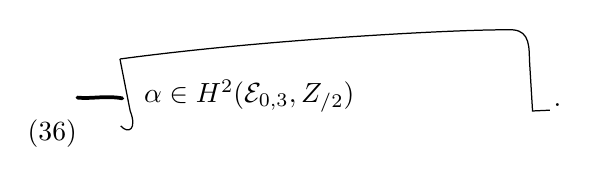
\begin{tikzpicture}[x=1cm,y=1cm,baseline=(formule.base)]
\node[anchor=west,inner sep=0pt] (formule) at (1.02,0)
  {$\alpha\in H^2(\mathcal E_{0,3},\mathbb Z_{/2})$};
\node[anchor=east,inner sep=0pt] at (0.18,-0.48) {$(36)$};
\draw[line width=0.45pt]
  (0.72,0.47) .. controls (2.65,0.73) and (5.13,0.85) .. (5.64,0.84)
  .. controls (5.89,0.86) and (5.92,0.70) .. (5.92,0.47)
  -- (5.96,-0.19) -- (6.18,-0.18);
\draw[line width=0.45pt]
  (0.72,0.47) -- (0.85,-0.19)
  .. controls (0.94,-0.42) and (0.83,-0.49) .. (0.73,-0.38);
\draw[line width=1.35pt,line cap=round]
  (0.18,-0.02) .. controls (0.35,-0.04) and (0.55,0.01) .. (0.75,-0.03);
\node[anchor=west,inner sep=0pt] at (6.22,-0.12) {.};
\end{tikzpicture}}
--- and nothing says that this cohomology class can be killed, by passing to an open subgroup of $\mathcal E_{0,3}$.
\figure{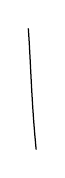
\begin{tikzpicture}[x=1cm,y=1cm]
\draw[line width=0.45pt]
  (0,1.05) .. controls (0.03,0.64) and (0.04,0.11) .. (0.10,-0.49);
\end{tikzpicture}}

\scanpage{526}

But in geometric terms, \deleted{\unsure{soon}} the relative elliptic curves \unsure{sought} over \unsure{$U_{0,2}$|$U_{0,3}$} form \unsure{\deleted{the}|the} sections of a stack over $(U_{0,3})_{\mathrm{et}}$, which is a \deleted{\unsure{$\{\pm1\}$}}\inserted{$\mathbb Z_{/2}$}-gerbe --- the obstruction therefore lies in a Brauer group
\[
\beta\in H^2(U_{0,3},\mathbb Z_{/2}), \tag{37}
\]
now since $U=U_{0,3}$ is an algebraic \deleted{\illegible{1}} affine curve over a field (it \unsure{would suffice} that it not be of type $0,0$) \unsure{it follows} that the canonical homomorphism (with arbitrary torsion coefficients)
\[
H^*(\mathcal E_U,-)\longrightarrow H^*(U,-)
\]
is an isomorphism. Besides, it \unsure{must} be $\pm$ trivial that $\beta$ is the image of $\alpha$ --- which confirms the \unsure{intuition|intention} that \deleted{\unsure{the}} if the lifting is possible at the level of profinite fundamental groups (\unsure{arithmetico-geometric|arithmetico-geometric}) it is also possible at the level of the modular \unsure{multiplicities} themselves, so that we have an existence of a relative elliptic curve over $U_{0,3}$ which\ldots

\scanpage{527}
\mspage{269}

It is \unsure{true} that it is well \unsure{known} that a cohomology class (37) with torsion coefficients is killed, on \unsure{passing} to a finite extension of the \deleted{\unsure{$\mathbb Q$}} base field ($\mathbb Q$ in this case). In fact, we have a spectral sequence
\[
(38)\qquad H^*(U_{0,3},\mathbb Z_{/2})
\Longleftarrow E_2^{pq}
=H^p(\deleted{\unsure{\overline U_{0,3}}}\unsure{\mathbb Q},H^q(\overline U_{0,3},\mathbb Z_{/2}\unsure{)|))}
\]
and here $H^q(\overline U_{0,3})=0$ for $q\geq 2$, so we find an exact sequence
\[
\deleted{\unsure{H^1(\mathbb Q)}\longrightarrow
\unsure{H^1(U_{0,3},\mathbb Z_{/2})}\longrightarrow
\unsure{H^1(\overline U_{0,3},-)}}
\]
\diagram{\begin{tikzcd}[ampersand replacement=\&,column sep=small,column sep=9pt,row sep=14pt,execute at begin picture={\fontsize{10}{12}\selectfont}]
\cdots \& E_2^{0,1} \arrow[r] \arrow[d,equal]
\& E_2^{2,0} \arrow[r] \arrow[d,equal]
\& \deleted{\unsure{E}}H^2(U_{0,3}) \arrow[r]
\& E_2^{1,1} \arrow[r] \arrow[d,equal]
\& E_2^{3,0} \arrow[d,equal] \& \cdots \\
\& H^0(\mathbb Q,H^1(\overline U)
\& H^2(\mathbb Q,\mathbb Z_{/2})
\&
\& H^1(\mathbb Q,\underset{\substack{\wr\\\mathbb F_2^2}}{H^1(\overline U)})
\& H^3(\mathbb Q,\unsure{\mathbb Z_{/2}|\mathbb F_2}) \&
\end{tikzcd}}

I \unsure{realize} at last that the existence of a \deleted{\illegible{1}} lifting, -- i.e. of the hypothetical elliptic curve over $U_{0,3}$ -- is completely trivial, it suffices to define \unsure{it|it} by the equation
\[
y=\sqrt{\unsure{x|\dot x}(x-1)(x-\lambda)}
\]
i.e.
\[
y^2-x(x-1)(x-\lambda)=F(x,y;\lambda]=0
\]
which defines an affine plane curve,
\scanpage{528}
\unsure{we pass|or pass} to projective coordinates
\[
F(x,y,z;\lambda)=y^2z-x^3+(1+\lambda)x^2z-\lambda xz^2=0
\]
\deleted{\unsure{for|then}} I am not going to go further into the question here\unsure{.} \unsure{to} what extent this choice is ``natural''.

\deleted{\unsure{Once}} \inserted{\unsure{It}} gives in any case a \unsure{homomorphis-}\deleted{\unsure{m outer}} \unsure{as} precise as can be
\[
(39)\qquad M_{0,4}^{!}=U_{0,3}\longrightarrow M_{1,1}
\]
hence a \unsure{homomorphism|homomorphism} of extensions
\diagram{\begin{tikzcd}[ampersand replacement=\&,column sep=small,row sep=small]
\& \& \widehat{\mathcal T}_{0,4}^{!+} \arrow[d,phantom,"\wr" description]
\& \unsure{N_{0,4}^{!}|\mathcal N_{0,4}^{!}} \arrow[d,phantom,"\wr" description] \& \& \\
(40) \& 1 \arrow[r]
\& \widehat\Pi_{0,3} \arrow[r] \arrow[d]
\& \mathcal E_{0,3} \arrow[r] \arrow[d]
\& \Gamma \arrow[r] \arrow[d,equal] \& 1 \\
\& 1 \arrow[r]
\& \widehat{\mathcal T}_{11}^{+} \arrow[r] \arrow[d,phantom,"\wr" description]
\& \mathcal E_{11} \arrow[r] \arrow[d,equal]
\& \Gamma \arrow[r] \& 1 \\
\& \& \unsure{\mathrm{Sl}}(2,\mathbb Z)^{\wedge}
\& \unsure{N_{1,1}|\mathcal N_{1,1}}\deleted{\unsure{\simeq\mathrm{Sl}(2,\mathbb Z)^{\wedge}}} \& \&
\end{tikzcd}}
defined modulo \unsure{automorphism|automorphism} \unsure{inner} by \deleted{and} an element of $\widehat{\mathcal T}_{11}^{+}\simeq\unsure{\mathrm{Sl}}(2,\mathbb Z)^{\wedge}$, and at the level of \unsure{discrete|discrete} groups
\[
\deleted{(41)}\qquad \Pi_{0,3}\longrightarrow\mathcal T_{1,1}^{+}
\]
\deleted{\unsure{but} it is no longer so very}
\inserted{and even}
\[
(42)\qquad \Pi_{0,3}\hookrightarrow
\overbrace{\operatorname{Ker}\left(
\underset{\substack{\Vert\\\unsure{\mathrm{Sl}}(2,\mathbb Z)}}{\mathcal T_{1,1}^{+}}
\longrightarrow
\underset{\substack{\Vert\\\unsure{\mathrm{Sl}}(2,\mathbb Z_{/2})}}{\unsure{\mathfrak S_3}}
\right)}^{\unsure{\Gamma_2}}
\]
(and ditto for the profinite groups). Here $\Pi_{0,3}$ is such that the congruence subgroup on the \unsure{second} \unsure{side|level} \deleted{\unsure{$\Gamma$}} i.e. $\unsure{\Gamma_2}$, \unsure{is|is} the direct product of \unsure{this|the} \unsure{subgroup|subgroups} $\Pi_{0,3}$ and of
\scanpage{529}
\mspage{270}
its center $\pm1$. (But in fact, there are \unsure{exactly} four subgroups of $\Gamma_2$ which \unsure{realize} this decomposition. So as not to make \unsure{anyone|anyone} jealous, one could look at the intersection of the four, which is a subgroup $\Gamma_2$ of index a divisor of $2^4=16$ it is the intersection of the kernels \unsure{of|of the} four homomorphisms $\Gamma_2\longrightarrow\deleted{\mathbb Z_{/2}}\ \unsure{\mathrm{Centre}}(\Gamma_2)=\{\pm1\}$,
\margin{\uline{N.B.} \unsure{That} must be the kernel of $\mathrm{Sl}(2,\mathbb Z)^{\unsure{\wedge|*}}\longrightarrow\mathrm{Sl}(2,\mathbb Z/4\mathbb Z)$}
As a subgroup of $\Pi_{0,3}$, its index is a divisor of $8$ -- It wouldn't surprise me if it were just the commutator group of $\Pi_{0,3}$,) which is of index $4$ -- there is a whole \unsure{situation} there to elucidate\ldots\,.
\margin{it is true and it is \unsure{$\simeq$|even} trivial\ldots}
\margin{It is not clear \deleted{whether $\Pi_{0,3}$} is invariant \unsure{as} a subgroup of \deleted{\unsure{$\mathfrak S$}} $\mathcal T_{1,1}^{+}\simeq\mathrm{Sl}(2,\mathbb Z)$, i.e. stable under the outer action of $\unsure{\mathfrak S}_3$ on $\mathrm{Sl}(2,\mathbb Z)$ -- I presume so, since $\unsure{\mathfrak S}_3$ also operates by outer automorphisms on $\Pi_{0,3}$ a priori\ldots\ $\mathcal T_{11}^{+}/\Pi_{0,3}$ would be an \unsure{interesting} central extension of $\unsure{\mathfrak S}_3$ by $\{\pm1\}$\ldots}

Of course, one should also make the homomorphism (42) explicit (defined \unsure{modulo} inner \unsure{automorphisms}) by its values on the generators $\unsure{l_0,l_1,l_2}$ -- I shall perhaps return to this later.

\scanpage{530}

\uline{Theorem} The natural outer action of $\Gamma_Q$ on $\widehat{\mathcal T}_{1,1}^{+}$, and even on $\widehat{\mathcal T}_{1,1}^{+\prime}=\widehat{\mathcal T}_{1,1}/(\pm1)$, is faithful.
\figure{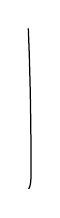
\begin{tikzpicture}[x=1cm,y=1cm]
\draw[line width=0.45pt]
  (0,1.05) .. controls (0.025,0.44) and (0.035,-0.19) .. (0.035,-0.78)
  .. controls (0.035,-0.91) and (0.025,-0.96) .. (0.005,-0.99);
\end{tikzpicture}}

We use the fact that we have an injective outer homomorphism
\[
\widehat{\Pi}_{0,3}\hookrightarrow\widehat{\mathcal T}_{1,1}^{\prime+}
\]
compatible with the action of $\Gamma$, proceeding as for the proposition at the beginning (where $\widehat{\Pi}_{0,3}'$ played the role of $\widehat{\mathcal T}_{1,1}^{\prime+}$).

\uline{Corollary} The canonical homomorphisms (surjective)
\[
\tag{43}
\Gamma_Q\longrightarrow\Gamma_{1,\nu}\qquad(\nu\geq1)
\]
are injective, hence isomorphisms.

It suffices to prove this for $\Gamma_Q\longrightarrow\Gamma_{1,1}$ (since $\Gamma_{1,1}$ is a quotient of $\Gamma_{1,\nu}$, $\nu\geq1\ldots$), now we have a homomorphism \unsure{\deleted{\illegible{1}}} $\Gamma_{1,1}\longrightarrow\mathrm{Aut\ ext}\,\widehat{\mathcal T}_{1,1}^{+}$ and we can consider the \unsure{composite}
